\section{Background and Related Work}
\label{sec:related-work}

Related work has been conducted in both of the main focus areas of this project:
the use of UI interaction data for security and implementing SDN on the Android
platform. We now review such work.

\subsection{UI Interaction and Security}
\label{sec:ui-interaction-and-security}

\begin{wrapfigure}{R}{0.4\textwidth}
	\centering
	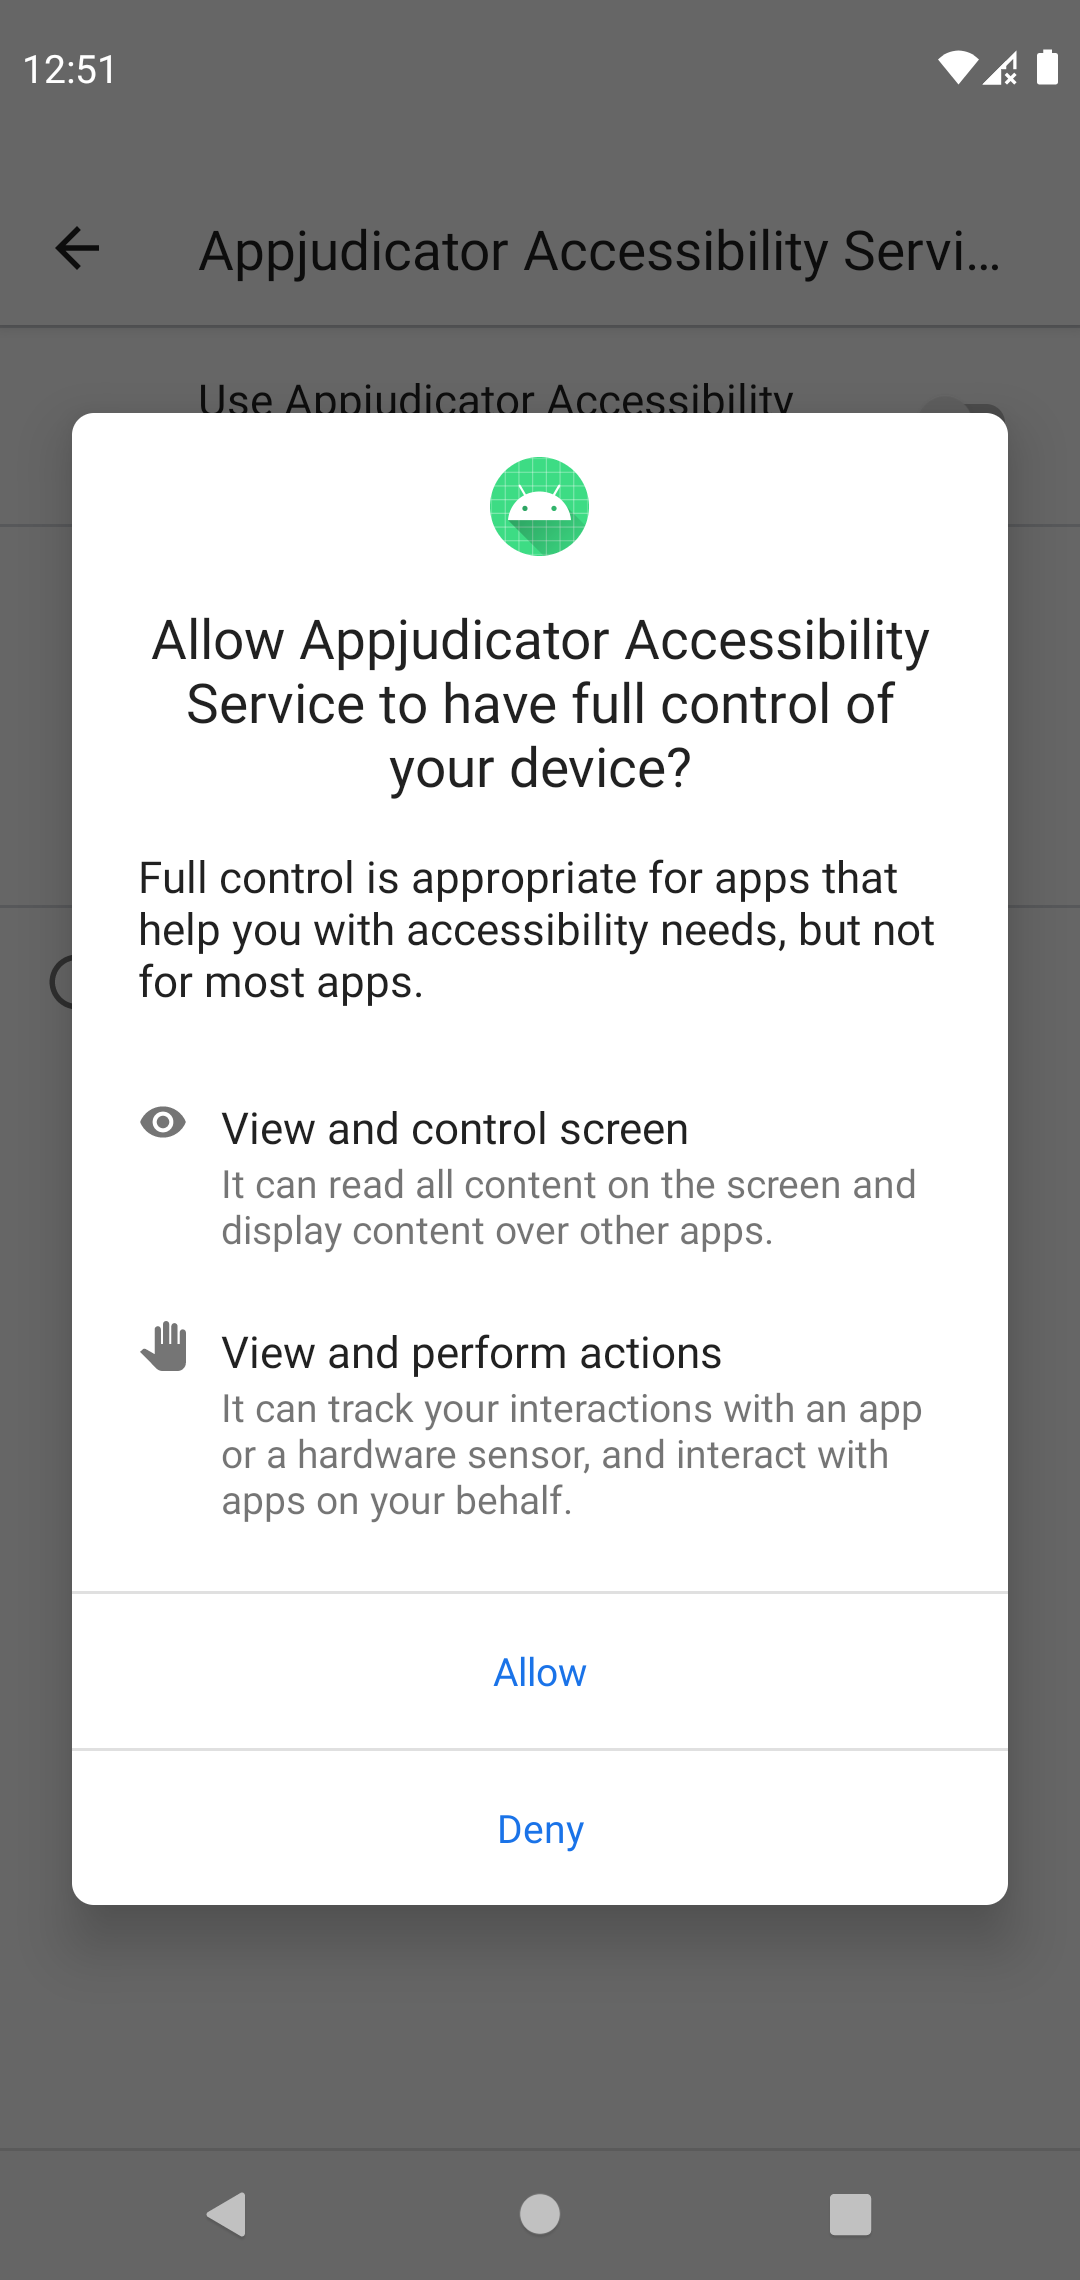
\includegraphics[width=0.4\textwidth]{a11y-warning-screenshot.png}
	\caption{Android displays this warning when enabling an accessibility
		service.}
	\label{fig:a11y-warning}
\end{wrapfigure}

Previous work has investigated how user interactions with the UI can be used to
identify human-initiated behavior on various platforms. Harbinger examines user
interface activity on Windows to provide context for network requests to
previously unknown hosts in a default-deny environment~\cite{chuluundorj2019}.
This approach ``hooks into'' mouse and keyboard inputs using Microsoft's UI
Automation library~\cite{microsoft2018}, intercepting the input before it is
received by the intended application. Although Harbinger's operations are
performed synchronously they still only added six milliseconds or less of
latency to 96\% of flows.\footnote{In contrast, the relevant Android library is
	asynchronous and event-driven~\cite{googledevelopers2020}.
	Section~\ref{sec:implementation-accessibility-service} discusses the
	benefits and challenges associated with this approach.}

Kwon \etal also used UI interaction data to distinguish human-generated from
automated network requests on Windows~\cite{kwon2011}. They propose a host-based
system for combating botnets by leveraging UI interaction data. But their
approach of labelling any flow initiated within one second of an interaction
with the flow's process as ``user generated'' ignores much of the context that
can be gained from UI data.

Shirley and Evans attempt to infer a users' intentions from their actions, and
define a language for writing access control policies based on these
intentions~\cite{shirley2008}. Their approach collects UI interactions like
mouse clicks and keystrokes, along with the state of the user interface. Like
other previous work mentioned above, they focus on Windows only, and use their
program to limit malware file access.

Cui \etal proposed a system called BINDER for Windows that attempts to detect
malicious network flows by associating user input events, process start and
finish events, and network events~\cite{cui2005}. Their system would only block
flows locally, and was never implemented. In contrast, our system integrates
into an SDN environment and provides context to network administrators.

% compare and contrast with this work.

\subsection{Android's Accessibility Service}
\label{sec:androids-accessibility-service}

Most previous work on Android has used the platform's
\texttt{AccessibilityService}, a library that includes the ability to respond to
UI changes among other accessibility features~\cite{googledevelopers2020}. Apps
that implement this API can be notified asynchronously of UI state transitions
in other all apps on the phone.

These services break the operating system's normally strong sandboxing
principles by their ability to read and interact with anything displayed on the
screen~\cite{kalysch2018, diao2019}. Real Android malware has taken advantage of
accessibility services to spy on users and take control of mobile
devices~\cite{kraunelis2013}. For security reasons, Android requires any
accessibility service to be enabled manually by the user in the settings app.
The operating system displays a dialog box to warn the user of the potential
security risks involved with accessibility services when one is first enabled
(see Figure~\ref{fig:a11y-warning}). Still, some have argued that even this
warning is not descriptive enough of the powerful and wide-reaching permissions
given to accessibility services~\cite{kalysch2018}.

Some prior work has been done on detecting malicious behavior using an
accessibility service. AppIntent~\cite{yang2013}, for example, uses this service
to determine if an app is leaking private information by building a graph of UI
interactions that could lead to information leakage. However, AppIntent is only
designed to determine whether an app \textit{could} leak private information
through static analysis and does not work in real time on a per-flow basis.

\subsection{Software-defined Networking}
\label{sec:software-defined-networking}

Software-defined networking (SDN) has been studied as a tool for giving network
administrators more information about, and control over, intra-network traffic.
In essence, SDN centralizes network intelligence by separating the forwarding of
packets (the data plane) from their routing (the control plane). In this
paradigm network switches merely forward packets, while all control and logic is
centralized with an SDN controller server~\cite{kim2013}.

The most commonly used SDN protocol is OpenFlow, a standard maintained by the
Open Networking Foundation~\cite{erickson2011}. The OpenFlow protocol provides a
standard way for SDN agents (usually network switches) to cache
packet-forwarding rules~\cite{openflowspec}. When a packet from a new flow
arrives at the agent, it looks up the most specific rule that applies to the
packet, then performs the actions listed in the rule. These actions can include
changing fields in the packet's header, forwarding it out a specific port, or
dropping the flow entirely. If the switch has no matching rule in its flow
table---or if a rule specifically requests it---the switch can forward the
packet in question to the central controller server to ask what to do with it.

SDN gives administrators more fine-grained control over packet routing rules,
which enables more sophisticated policy enforcement. It also provides insight
into potential issues and congestion in the network from one centralized control
point, rather than spread across many switches and routers. The main drawback of
this approach is the high overhead that causes it to scale
poorly~\cite{benzekki2016}.

Several techniques for distributing the load on the controller server have been
tried~\cite{oktian2017, dixit2013}. Some authors have investigated using end
nodes, instead of routers and switches, as SDN rule caches to alleviate this
problem~\cite{taylor2017, chuluundorj2019}. In this approach, each host caches
rules from the SDN controller and makes routing decisions about its own network
flows. \textsc{Appjudicator} follows this strategy, implementing a host-based
SDN agent and extending the OpenFlow protocol with more context.

Taylor ~\etal explores the feasibility of separating the SDN controller from the
local network entirely, connecting instead to a cloud-based
controller~\cite{taylor2017shue}. They were able to achieve acceptable overhead
for 90\% of end users by selecting low-latency public cloud locations.

Others have investigated the potential for improving SDN's capabilities by
adding context~\cite{yang2015}, an approach which \textsc{Appjudicator} also
attempts. SDN rules could be more powerful and granular with more metadata, for
example a network flow's initiating application.

Qazi \etal attempts to classify traffic from Android phones using machine
learning on an SDN switch~\cite{qazi2013}. Their approach achieves 94\%
accuracy in the top 40 Android applications. By utilizing the phone itself as
an SDN agent \textsc{Appjudicator} is able to identify a network flow's
originating application with 100\% accuracy.

\subsection{The Android Phone as an SDN Agent}
\label{sec:the-android-phone-as-an-sdn-agent}

Several previous applications have used an Android smartphone as a SDN agent and
rule cache. Hong~\etal explores the tools available to organizations for
managing BYOD Android devices and proposes a system for applying SDN policies to
these phones~\cite{hong2016}. They were able to apply app-specific rules that
were aware of device context such as GPS location with low overhead. However,
this work does not take advantage of the many extra sources of context the
mobile device can provide.

While Hong~\etal \cite{hong2016} and \textsc{Appjudicator} are both aimed at
corporate users, HanGuard investigated using SDN principles to protect Internet
of things (IoT) devices in home networks~\cite{demetriou2017}. Their application
provided tools for users to easily define SDN rules for IoT apps, IoT devices,
and users.

While each of these areas has been extensively researched alone, only
Chuluundorj~\cite{chuluundorj2019} and Kwon~\etal \cite{kwon2011} have
investigated how UI and network data can be combined for security purposes.
However, both of these applications were developed for the Windows
platform---bringing the idea to Android involves a new set of constraints and
challenges. For example, our proposed solution can be installed as a normal app,
and does not require recompiling the kernel or rooting the phone. This means
that we cannot modify the operating system kernel as the Windows solutions do,
and must abide by Android's strict permissions system.

\newpage

